\documentclass[reprint,english]{revtex4-1}

% language
\usepackage[utf8]{inputenc}
\usepackage[english]{babel}

% standard setup
\usepackage{physics,amssymb,array}
\usepackage{xcolor,graphicx,hyperref}
\usepackage{tikz,listings,multirow,caption}
\usepackage{algpseudocode,algorithm}
\usepackage{subfigure}
\usepackage{enumitem}

% hyperref coloring
\hypersetup{ %
  colorlinks,
  linkcolor={red!50!black},
  citecolor={blue!50!black},
  urlcolor={blue!80!black}}

% lstlisting coloring
\lstset{ %
  inputpath=,
  backgroundcolor=\color{white!88!black},
  basicstyle={\ttfamily\scriptsize},
  commentstyle=\color{magenta},
  language=C++,
  tabsize=2,
  stringstyle=\color{green!55!black},
  frame=single,
  keywordstyle=\color{blue},
  showstringspaces=false,
  columns=fullflexible,
  keepspaces=true}

% no "do"'s
\algdef{SE}[FOR]{NoDoFor}{EndFor}[1]{\algorithmicfor\ #1}{\algorithmicend\ \algorithmicfor}
\algdef{SE}[FORALL]{NoDoForAll}{EndFor}[1]{\algorithmicfor\ #1}{\algorithmicend\ \algorithmicfor}
\algdef{SE}[IF]{NoThenIf}{EndIf}[1]{\algorithmicif\ #1}{\algorithmicend\ \algorithmicif}

% pretty matrix
\newcolumntype{C}[1]{>{\centering\arraybackslash$}p{#1}<{$}}

% simplify
\newcommand{\Ham}{\hat{\mathcal{H}}}

\begin{document}
% titlepage
\title{FYS3150 Report\\Project 3 : Gravitational \(N\)-Body Simulation}
\author{Nils Johannes Mikkelsen}
\date{\today}
\noaffiliation
\begin{abstract}
Gravitational \(N\)-body systems are analysed using the initial condition numerical integration methods Forward-Euler and Velocity-Verlet. The Velocity-Verlet method is found easily superior to the low-order Forward-Euler method. The systems studied include the Newtonian systems: \emph{Earth-Sun}, \emph{Earth-Jupiter-Sun} and the complete \emph{Solar System}, and the relativistic system \emph{Mercury-Sun}. The focus lies on circular orbits, perturbations of circular orbits as well as escape velocity, numerical stability and perihelion precession due to relativistic effects.
\end{abstract}
\maketitle

% body
\section*{About Project 3}
This is a report for Project 3 in FYS3150 Computational Physics at UiO, due October \(24^{\text{st}}\), 2018. \cite{project3}
The project description was accessed October \(15^{\text{th}}\), 2018 with the following web address:\\
{\scriptsize\url{http://compphysics.github.io/ComputationalPhysics/doc/Projects/2018/Project3/pdf/Project3.pdf}}\\
All material written for this report can be found in this GitHub repository:\\
{\scriptsize\url{https://github.com/njmikkelsen/comphys2018/tree/master/Project3}}
\section{Introduction}
The aim of this project is to use numerical integration in order to study the gravitational \(N\)-body problem, in particular our Solar System. The problem will be disected into smaller components in order to isolate the effects between the gravitational objects. The first system (or component) to be studied is the isolated Earth-Sun system: it serves mainly as a classification of the numerical methods and to study how gravity behaves with respect to numerical algorithms. Next, Jupiter is added to the Earth-Sun system so that the perturbations of planetary orbits may be studied in isolation. Then, finally all planets are added to the system and simulated with all planet-planet gravitational effects included.

As a final challenge, a relativistic correction is added to the gravitational acceleration such that the observed perihelion precession of Mercury may be studied. The perihelion precesses by as little as 43'' per century, meaning this system serves as a good estimator for whether the numerical algorithms are stable in the long run.
\section{Theory}
\subsection{On The Physics of Gravitational Systems}
The main focus in Project 3 lies on 4 different gravitational systems: Three Newtonian systems with 2, 3 and \(N\) bodies, and one relativistic system with 2 bodies.
\subsubsection{The general problem statement}
Assuming an inertial frame of reference with \(J\) rigid objects not in contact, the net force on object \(j\in\{1,\ldots,J\}\) may be decomposed into gravitational effects and all other effects:
\begin{equation}\label{eq:general_net_force}
\vb{F}_\text{net}^j=\sum_{k\neq j}^J\Big(\vb{G}^{kj}+\vb{F}_\text{add}^j\Big)
\end{equation}
where \(\vb{G}^{kj}\) is the gravitational force from object \(k\) on \(j\) and \(\vb{F}_\text{add}^j\) includes all additional forces on object \(j\) such as electromagnetic radiation etc. The contributions from \(\vb{F}_\text{add}^j\) are miniscule compared to gravity and will therefore be ignored in this report.

Using Newtonian gravity, the gravitational force \(\vb{G}^{kj}\) is
\begin{equation}\label{eq:newtonian_gravity}
\vb{G}^{kj}=GM_jM_k\frac{\delta\vb{r}^{kj}}{\,|\delta\vb{r}^{kj}|^3}
\end{equation}
where \(G\) is the \emph{universal gravitational constant}, \(M_j\) and \(M_k\) are the masses of objects \(j\) and \(k\) respectively, and \(\delta\vb{r}^{kj}=\vb{r}^k-\vb{r}^j\) is the position of object \(k\) relative to the position of object \(j\). Following Newton's second law, the gravitational acceleration \(\vb{g}^{kj}\) experienced by object \(j\) due to \(\vb{G}^{kj}\) is simply
\begin{equation}\label{eq:newtonian_gravitational_acceleration}
\vb{g}^{kj}=\frac{\vb{G}^{kj}}{M_j}=GM_k\frac{\delta\vb{r}^{kj}}{\,|\delta\vb{r}^{kj}|^3}
\end{equation}
Therefore in a Newtonian system, the net gravitational acceleration experienced by object \(j\) due to the other objects is given by rewriting equation \eqref{eq:general_net_force} using Newton's second law and inserting \eqref{eq:newtonian_gravitational_acceleration}:
\begin{equation}\label{eq:net_newtonian_gravitational_acceleration}
\vb{g}^j=G\sum_{k\neq j}^JM_k\frac{\delta\vb{r}^{kj}}{\,|\delta\vb{r}^{kj}|^3}
\end{equation}

Invoking General Relativity, the concept of a gravitational force is replaced by the curvature of spacetime. However, the Newtonian jargon may be continued by introducing a relativistic correction to the Newtonian expression for gravitational acceleration:
\begin{equation}\label{eq:relativistic_gravitational_acceleration}
\vb{g}_\text{rel}=\vb{g}_\text{N}\,\Bigg[1+3\frac{|\vb{r}\times\vb{v}|^2}{|\vb{r}|^2c^2}\Bigg]
\end{equation}
where \(\vb{g}_\text{rel}\) and \(\vb{g}_\text{N}\) is the relativistic and Newtonian acceleration, \(\vb{r}\) and \(\vb{v}\) are the position and velocity, and \(c\) is the speed of light. Hence, the relativistic version of equation \eqref{eq:net_newtonian_gravitational_acceleration} is
\begin{equation}\label{eq:net_relativistic_gravitational_acceleration}
\vb{g}^j=G\Bigg[1+3\frac{|\vb{r}^j\times\vb{v}^j|^2}{|\vb{r}^j|^2c^2}\Bigg]\sum_{k\neq j}^JM_k\frac{\delta\vb{r}^{kj}}{\,|\delta\vb{r}^{kj}|^3}
\end{equation}

In conclusion, in order to simulate the movement of Newtonian/relativistic gravitational objects, the following set of simultaneous second order differential equations must be solved:
\begin{subequations}\label{eq:main_problem}
\begin{align}
\text{Newtonian:}&\nonumber\\
\dv[2]{t}\vb{r}^j&=G\sum_{k\neq j}^JM_k\frac{\delta\vb{r}^{kj}}{\,|\delta\vb{r}^{kj}|^3}\\
\text{Relativistic:}&\nonumber\\
\dv[2]{t}\vb{r}^j&=G\Bigg[1+3\frac{|\vb{r}^j\times\vb{v}^j|^2}{|\vb{r}^j|^2c^2}\Bigg]\sum_{k\neq j}^JM_k\frac{\delta\vb{r}^{kj}}{\,|\delta\vb{r}^{kj}|^3}
\end{align}
\end{subequations}
for all \(j\in\{1,\ldots,J\}\), provided an appropriate set of initial conditions \(\{t_0,\vb{r}^j(t_0),\vb{v}^j(t_0)\}_ j\) for each object.
\subsubsection{Experimental gravity}
Seeing that the \(1/r^2\) dependence of the gravitational acceleration is particular to Newtonian gravity, it is tempting to analyse a generalised dependence \(1/r^\beta\). Clearly for \(\beta\) values slightly greater than 2, the gravitational pull from the Sun on the planets would just fail to stabilise the planets' kinetic energy, leaving the planets slowly drift away. For \(\beta\) values slightly less than 2, the orbits are likely to remain stable despite loosing their original approximately-elliptic shape. Introducing such a generalised dependence is easy, instead of the \(1/|\delta\vb{r}^{kj}|^3\) dependence in \eqref{eq:newtonian_gravitational_acceleration}, the gravitational acceleration would instead have a \(1/|\delta\vb{r}_{kj}|^{\beta+1}\) dependence:
\begin{equation}\label{eq:beta_Newtonian_gravitational_acceleration}
\vb{g}^{kj}(\beta)=GM_k\frac{\delta\vb{r}^{kj}}{\,|\delta\vb{r}^{kj}|^{\beta+1}}
\end{equation}
The equivalent net "\(\beta\)-Newtonian" gravitational acceleration is then found as before: \(\vb{g}^j(\beta)=\sum_{k\neq j}^J\vb{g}^{kj}(\beta)\).
\subsubsection{Units}
Knowing that the simulations will take place on the scale of the solar system, it is computationally expensive to use SI units. The simulations will therefore be run using the so-called astronomical, or au, system of units. This system of units is inspired by Earth's orbit about the Sun and thus defines the unit of time and space according to the period and average radius of the orbit. The unit of length is the astronomical unit au, which today is defined exactly as 1 au\(\,=149\,597\,870\,700\) m. The unit of time is the Julian year, i.e. \(365.25\) days\(\,=31\,557\,600\) s.

The astronomical units is not a strictly closed system in that several units of mass are used, this report will use the most computationally friendly one: the solar mass 1 \(\text{M}_\odot=1.988500\cdot10^{30}\) kg.

From the unit definitions of length and time, the speed of light in a vacuum \(c\) can be expressed in astronomical units as
\begin{equation}\label{eq:light_speed_au_units}
c=299 792 458\text{ m/s}\cong63241.08\text{ au/yr}
\end{equation}

Using the unit definitions for length, time and mass, the universal gravitational constant can be expressed in astronomical units as
\begin{subequations}\label{eq:G_au_units}
\begin{align}
G&=6.67408\cdot10^{-11}\text{ m}^3\text{ s}^{-2}\text{ kg}^{-1}\\
&\cong39.4774\text{ au}^3\text{ yr}^{-2}\ M_\odot^{-1}
\end{align}
\end{subequations}
It is not a coincidence that the value for \(G\) in au units is approximately equal to \(4\pi^2\), Kepler's \(3^\text{rd}\) Law of two-body orbits states that the semi-major axis \(a\) of an elliptical orbit is proportional to the square of the orbital period \(T\):
\begin{equation}\label{Kepler_3rd_law}
\frac{a^3}{T^2}=\frac{G(M_1+M_2)}{4\pi^2}
\end{equation}
where \(M_1\) and \(M_2\) are the masses of the bodies involved. For the Earth-Sun system, \(a^3/T^2=1\text{ au}^3/\text{ yr}^2\) and \(M_\odot+M_\text{Earth}\approx M_\odot\) so that \(G=4\pi^2\text{ au}^3\text{ yr}^{-2}\ M_\odot^{-1}\).
\subsubsection{Circular orbit}
Assuming a single gravitational body with mass \(m\) is orbiting a massive object with mass \(M\) whose motion is negligible, the gravitational acceleration would equal the centripetal acceleration of the body:
\[m\frac{{v_\text{circ}}^2}{R}=\frac{GmM}{R^2}\]
where \(v_\text{circ}\) is the orbital speed of orbiting body. When rearranged, this yields the orbital speed as a function of the orbit radius and mass of the massive object:
\begin{equation}\label{eq:circular_orbital_speed}
v_\text{circ}=\sqrt{\frac{GM}{R}}
\end{equation}
\subsubsection{Planetery escape velocity}
In the unlikely event that a planet and the Sun is isolated, and the planet is given escape velocity in the direction radially outwards from the Sun, consevation of energy would imply that the planet's initial kinetic energy would equal the total work done by the Sun on the planet. The work done needed for the planet to escape the Sun (meaning travel infinitely far away without external forces acting on Earth during the journey) starting from a distance \(R\) is given by
\begin{align}
W_\text{esc}&=-\int_{\mathcal{C}_R}\dd{\vb{r}}\frac{-GM_pM_\odot}{|\vb{r}|^3}\vb{r}=GM_pM_\odot\int_R^\infty\frac{\dd{r}}{r^2}\nonumber\\
&=-GM_pM_\odot\frac{1}{r}\eval_R^\infty=-GM_pM_\odot\Big(0-\frac{1}{R^2}\Big)\nonumber\\
W_\text{esc}&=\frac{GM_pM_\odot}{R}
\end{align}
where \(M_p\) is the planet's mass and \(\mathcal{C}_R\) is a straight curve starting a distance \(R\) from the origin and directed radially outwards from the Sun. The initial kinetic energy of the planet is \(K_\text{esc}=\frac{1}{2}M_p{v_\text{esc}}^2\), hence the escape velocity of the planet is given by
\begin{equation}\label{eq:escape_velocity}
W_\text{esc}=K_\text{esc}\implies v_\text{esc}=\sqrt{2\frac{GM_\odot}{R}}
\end{equation}
\subsubsection{The perihelion precession of the planets}
The French mathematician Urbain Le Verrier discovered in the mid-\(19^\text{th}\) century that the perihelion (the point on a planetary orbit that is closest to the Sun) of Mercury, in direct violation with contemporary Newtonian celestial mechanics, precessed about Solar System's planar axis. The angular velocity of the precession, which was not fully explained until the advent of general relativity, measures a tiny 43'' per century. Using the relativistic correction in \eqref{eq:net_relativistic_gravitational_acceleration}, the precession should be reproduceable. The distance from Mercury to the Sun and the orbital speed of Mercury at perihelion is 0.3075 AU and 12.44 AU/yr respectively.
\subsection{Numerical integration - Initial Value Problems}
The following theory is based on Lectures in FYS-3150. \cite{lecture_ode}

The problem at hand (equation \eqref{eq:main_problem}) is a so-called differential equation initial value problem. An analytic solution does in general not exist, meaning numerical methods are necessary. This report will introduce two integration methods (or schemes), the Forward-Euler method and the Velocity-Verlet method.
\subsubsection{Preliminary}
In order to maintain some level of generality, both methods will be discussed in the absence of knowledge of the gravitational acceleration. Newton's second law of motion is second order ordinary differential equation, which in the most general case may be written as
\begin{equation}\label{eq:second_order_diff_eq}
\vb{f}''(t)=\dv[2]{\vb{f}}{t}\big(t,\vb{f}(t),\vb{f}'(t)\big)
\end{equation}
where \(\vb{f}(t)\) is the solution in question and \(\dv*[2]{\vb{f}}{t}\) is a known function. To avoid having to write out \(\vb{f}(t)\), its derivatives, etc., the following will introduce a simplified notation.

Let \(t_i\) denote the \((i+1)^\text{th}\) element in the linearly spaced set of \(t\) values:
\begin{equation}
\left\{t_i=t_0+ih\ :\ i\in\mathbb{Z}^+,\,t_0\in\mathbb{R},\,h\in\mathbb{R}^+\right\}
\end{equation}
Furthermore, define \(\vb{f}_i=\vb{f}(t_i)\) and let prime-notation, e.g. \(\vb{f}'\), denote taking the derivative with respect to \(t\).

Using this notation, the first- and second-order taylor expansion of \(\vb{f}\) about \(t_i\), evaluated at \(t_{i+1}\), is simply
\begin{subequations}\label{eq:general_taylor_expansion}
\begin{align}
\vb{f}_{i+1}&=\vb{f}_i+h\vb{f}'_i+\order{h^2}\\
\vb{f}_{i+1}&=\vb{f}_i+h\vb{f}'_i+\frac{h^2}{2}\vb{f}''_i+\order{h^3}
\end{align}
\end{subequations}

In case \(\vb{f}\) represents the position vector \(\vb{r}\), the derivatives \(\vb{r}'\) and \(\vb{r}''\) are simply the velocity and acceleration vectors \(\vb{r}\) and \(\vb{a}\). In case \(\vb{f}\) represents the velocity vector \(\vb{v}\), the derivatives \(\vb{v}'\) and \(\vb{v}''\) represent the acceleration and the derivative of the acceleration vectors \(\vb{a}\) and \(\vb{a}'\).
\subsubsection{Forward-Euler}
The Forward-Euler integration scheme is a low-order, somewhat inaccurate, integration method originating from some of the earliest and most tedius attempts of numerical calculus. The method has been included for exactly this reason: namely to highlight the difference in accuracy between different integration methods.

The Forward-Euler scheme is easy to outline, it follows exactly from the first-order taylor expansions of \(\vb{r}\) and \(\vb{v}\):
\begin{subequations}\label{eq:forward_euler_method}
\begin{align}
\vb{r}_{i+1}&=\vb{r}_i+h\vb{v}_i+\order{h^2}\\
\vb{v}_{i+1}&=\vb{v}_i+h\vb{a}_i+\order{h^2}
\end{align}
\end{subequations}
Note that the order-terms are ignored in the integration. Each step in a Forward-Euler integration carries an error of order \(h^2\), thus with \(N\) steps the global error made in an integration is equal to \(N\order{h^2}\). It is customary to let \(t\) run from \(t=0\) to some \(t=t_N=Nh\) so that the global error may be written as \(t_N\order{h}\).
\subsubsection{Velocity-Verlet}
The Velocity-Verlet method is a second-order integration scheme that, as the name implies, focuses on the velocity. The method is energy-conservative in that if \(\vb{r}\) and \(\vb{v}\) represents the position and velocity of an object in an inertial frame of reference, its total mechanical energy would be conserved in time.

The Velocity-Verlet method follows from the second-order taylor expansions of \(\vb{r}\) and \(\vb{v}\):
\begin{subequations}
\begin{align}
\vb{r}_{i+1}&=\vb{r}_i+h\vb{v}_i+\frac{h^2}{2}\vb{a}_i+\order{h^3}\\
\vb{v}_{i+1}&=\vb{v}_i+h\vb{a}_i+\frac{h^2}{2}\vb{a}'_i+\order{h^3}
\end{align}
\end{subequations}
The term \(\vb{a}'_i\) is now approximated using a first-order taylor expansion of \(\vb{a}_i\):
\[\vb{a}_{i+1}=\vb{a}_i+h\vb{a}'_i+\order{h^2}\]
such that
\[\vb{a}'_i=\frac{\vb{a}_{i+1}-\vb{a}_i}{h}+\order{h}\]
Inserting into the above equations thus yields
\begin{subequations}
\begin{align}\label{eq:velocity_verlet_method}
\vb{r}_{i+1}&=\vb{r}_i+h\vb{v}_i+\frac{h^2}{2}\vb{a}_i+\order{h^3}\\
\vb{v}_{i+1}&=\vb{v}_i+\frac{h}{2}\Big[\vb{a}_i+\vb{a}_{i+1}\Big]+\order{h^3}
\end{align}
\end{subequations}
Unlike the Forward-Euler method, the Velocity-Verlet method is invalid for accelerations dependent on velocity: note in particular that \(\vb{v}_{i+1}\) is dependent on \(\vb{a}_{i+1}\). In case the acceleration is dependent on the position (such as in the case of gravitational acceleration), the position vector \(\vb{r}_{i+1}\) must be evaluated before \(\vb{v}_{i+1}\). That is, the Velocity-Verlet method is order-specific with respect to evaluating \(\vb{r}_{i+1}\) and \(\vb{v}_{i+1}\) for accelerations dependent on position. The global error made in a Velocity-Verlet integration is \(N\order{h^3}=t_N\order{h^2}\).
\section{Method}
\subsection{Algorithms}
Having introduced the integration methods in the theory section, this section will take a step further and discuss the actual algorithms used in the simulations. That is, implementing the Forward-Euler and Velocity-Verlet methods as an algorithm for integrating the gravitational \(N\)-body problem.

In the following sections, exactly \emph{how} to compute the gravitational acceleration \(\vb{g}_i^j=\vb{g}^j(t_i)\) is momentarily ignored as it is treated later.
\subsubsection{Static/Stationary objects}
It is not uncommon that a particular object in a simulation barely moves, e.g., the Sun in the Sun-Earth system. More often that not, the movement of such an object has no impact on the results, meaning no important details are lost by ignoring it. Therefore, this project will divide gravitational objects into dynamic bodies and static (or stationary) bodies. In order to differentiate between dynamic and static objects, the complete set of object indices \(\{1,\ldots,J\}\) is divided into two subsets \(J_\text{dyn}\) and \(J_\text{stat}\), containing the indices corresponding to dynamic and static indices respectively.

The introduction of static bodies may significantly reduce the number of computations per simulation. This would not only improve the programs' efficiency with respect to program run-time, but it may also reduce the risk of accumulating floating point errors.
\subsubsection{Forward-Euler integration}
The first method is the Forward-Euler integration method, which is in fact particularly easy to implement: the next position and velocity vectors \(\vb{r}_{i+1}\) and \(\vb{v}_{i+1}\) can be computed directly as stated in equations \eqref{eq:forward_euler_method}. Hence, for a complete Forward-Euler integration with \(N\) steps of time-step \(h\), the algorithm may be written as:
\begin{algorithm}[H]
\caption{Forward-Euler integration}\label{alg:Forward_Euler}
\begin{algorithmic}[1]
\State Set initial condition \(t_0\).
\NoDoFor {\(j\in J_\text{dyn}\):}
	\State Set initial conditions \(\vb{r}_0\) and \(\vb{v}_0\) for object \(j\).
\EndFor
\NoDoFor {\(i\in\{0,\ldots,N\}\):}
	\NoDoFor {\(j\in J_\text{dyn}\):}
		\State Compute \(\vb{g}_i^j\).
		\State Compute \(\vb{r}_{i+1}^j=\vb{r}_i^j+h\vb{v}_i^j\).
		\State Compute \(\vb{v}_{i+1}^j=\vb{v}_i^j+h\vb{a}_i^j\).
	\EndFor
\EndFor
\end{algorithmic}
\end{algorithm}
Note that in the actual implimentation of Algorithm \ref{alg:Forward_Euler}, the gravitational acceleration \(\vb{g}_i^j\) is computed for each \(j\in J_\text{dyn}\) before updating the position and velocities: \(\vb{r}_{i+1}^j\) and \(\vb{v}_{i+1}^j\). This is simply a result of the specific program structure and has no effect on the results. This comment is included for clarity.
\subsubsection{Velocity-Verlet integration}
The second method is the Velocity-Verlet integration method. The basic principle behind Algorithm \ref{alg:Forward_Euler} carries over to the Verlet algorithm, however, the inclusion of \(\vb{g}_{i+1}^j\) in the calculation of \(\vb{v}_{i+1}^j\) poses an additional challenge. The gravitational acceleration is dependent on position, thus \(\vb{r}_{i+1}^j\) must computed before \(\vb{v}_{i+1}^j\). However, it would be rash to compute both \(\vb{g}_i^j\) and \(\vb{g}_{i+1}^j\) at each step, seeing that \(\vb{g}_{i+1}^j\) eventually becomes \(\vb{g}_i^j\) in the next step. For a complete Velocity-Verlet integration with \(N\) steps of time-step \(h\), the algorithm can be written as:
\begin{algorithm}[H]
\caption{Velocity-Verlet integration}\label{alg:Velocity_Verlet}
\begin{algorithmic}[1]
\State Set initial condition \(t_0\).
\NoDoFor {\(j\in J_\text{dyn}\):}
	\State Set initial conditions \(\vb{r}_0\) and \(\vb{v}_0\) for object \(j\).
	\State Compute \(\vb{g}_0^j\).
\EndFor
\NoDoFor {\(i\in\{0,\ldots,N\}\):}
	\NoDoFor {\(j\in J_\text{dyn}\):}
		\State Compute \(\vb{g}_{i+1}^j\).
		\State Compute \(\vb{r}_{i+1}^j=\vb{r}_i^j+h\vb{v}_i^j+\frac{1}{2}h^2\vb{g}_i^j\).
		\State Compute \(\vb{v}_{i+1}^j=\vb{v}_i^j+\frac{1}{2}h\big(\vb{g}_i^j+\vb{g}_{i+1}^j\big)\).
		\State Set \(\vb{g}_i^j=\vb{g}_{i+1}^j\).
	\EndFor
\EndFor
\end{algorithmic}
\end{algorithm}
Again, note that the actual implementation of Algorithm \ref{alg:Velocity_Verlet} is slightly different due to program structure: Here, the position is first updated using \(\vb{g}_i^j\), next \(\vb{g}_{i+1}^j\) is computed such that finally \(\vb{v}_{i+1}^j\) may be computed. This comment is included for clarity.
\subsubsection{Evaluating the gravitational acceleration}
Regardless of the chosen integration method, the gravitational acceleration on each dynamic object from every other object needs to be computed at every time step. Consider first the simplest case: standard Newtonian gravity (equation \eqref{eq:net_newtonian_gravitational_acceleration}). The following algorithm loops over each object and computes its contribution to the net gravitational acceleration on object \(j\):
\begin{algorithm}[H]
\caption{Computing the Newtonian \(\vb{g}_i^j\).}\label{alg:newtonian_gravity}
\begin{algorithmic}[1]
\State Initiate \(\vb{g}^j=\vb{0}\).
\NoDoFor {object \(k\in\{1,\ldots,N\}\):}
	\NoThenIf {\(k\neq j\):}
		\State \(\delta\vb{r}_i^{kj}=\vb{r}_i^k-\vb{r}_i^j\).
		\State \(\vb{g}_i^j\mathrel{{+}{=}}M_k\delta\vb{r}_i^{kj}/|\delta\vb{r}_i^{kj}|^3\).
	\EndIf
\State \(\vb{g}_i^j\mathrel{{*}{=}}G\)
\EndFor
\end{algorithmic}
\end{algorithm}
In order to extend Algorithm \ref{alg:newtonian_gravity} to the relativistic case, only a simple adjustment is necessary:
\captionsetup[algorithm]{labelformat=empty}
\begin{algorithm}[H]
\caption{\textbf{Adjustment} Relativistic correction to \(\vb{g}_i^j\).}\label{alg:newtonian_gravity}
\begin{algorithmic}
\State \(\vb{g}_i^j\mathrel{{*}{=}}G\Big[1+3|\vb{r}_i^j\times\vb{v}_i^j|^2/(|\vb{r}_i^j|^2c^2)\Big]\)
\end{algorithmic}
\end{algorithm}
Similarly, extending Algorithm \ref{alg:newtonian_gravity} to the \(\beta\)-Newtonian case requires only the following adjustment:
\begin{algorithm}[H]
\caption{\textbf{Adjustment} \(\beta\)-Newtonian correction to \(\vb{g}_i^j\).}\label{alg:newtonian_gravity}
\begin{algorithmic}
\State \(\vb{g}_i^j\mathrel{{+}{=}}M_k\delta\vb{r}_i^{kj}/|\delta\vb{r}_i^{kj}|^{\beta+1}\).
\end{algorithmic}
\end{algorithm}
\subsection{Simulations}
The following section presents the various scenarios simulated in this project.
\subsubsection{The Earth-Sun system}
The first system to be simulated is the simple two-body Earth-Sun system. Initially, Earth will placed in a circular orbit in order to assess the stability of the two integration algorithms as a function of different time step lengths \(h\). The Sun is categorised as a static body located at the origin. To simplify, Earth is placed at \(\vb{r}_0=(1,0,0)\) au with velocity \(\vb{v}_0^\text{Earth}=(0,v_\text{circ}^\text{Earth},0)\), where equation \eqref{eq:circular_orbital_speed} with \(M=M_\odot=1\) and \(R=1\) au yields an orbital speed of \(v_\text{circ}^\text{Earth}=2\pi\) au/yr.

As an ideal orbit would have \(|\vb{r}_i|=1\) for all \(i\), the standard deviation in \(|\vb{r}|\) will be used as a measure for the stability of the results. Additionally, knowing that the Velocity-Verlet algorithm is energy-conservative, stability will also be evaluated using the standard deviation in the mechanical energy \(E\) and angular momentum \(\vb{L}\):
\begin{subequations}
\begin{align}
E&=K+U=\frac{1}{2}M_E|\vb{v}|^2-\frac{GM_EM_\odot}{|\vb{r}|}\label{eq:mechanical_energy}\\
|\vb{L}|&=|\vb{r}\times M_E\vb{v}|\label{eq:angular_momentum}
\end{align}
\end{subequations}
Note however that the only action of \(M_E\) in the above equations is to scale the values. Hence, the underlying conserved quantites are actually
\begin{subequations}
\begin{align}
\frac{E}{M_E}&=\frac{1}{2}|\vb{v}|^2-\frac{GM_\odot}{|\vb{r}|}\\
l&=|\vb{r}\times\vb{v}|
\end{align}
\end{subequations}
The Velocity-Verlet algorithm is bound to produce better results than the Forward-Euler algorithm. In all remaining the simulations, only the Veloicty-Verlet algorithm will be used.

Having checked the stability of the algorithms, the escape velocity of Earth will be studied. Again the Sun is static at the origin and the origin is placed at \(\vb{r}_0=(1,0,0)\) au, now however with initial velocity \(\vb{v}_0^\text{Earth}=(v_\text{esc}^\text{Earth},0,0)\). Using astronomical units and \(R=1\) au, equation \eqref{eq:escape_velocity} yields \(v_\text{esc}^\text{Earth}=2\sqrt{2}\pi\) au/yr. Although this is perfect for the ideal system, numerical errors may affect the simulated escape velocity to a small degree. In order to test the accuracy of the simulated escape velocity, the simulation will be run using a small dense set of normally distributed velocities, centered about the ideal escape velocity.

Furthermore, it is of academic interest to study the same problem with the standard Newtonian gravity replaced by the general \(\beta\)-Newtonian gravity. Earth will be given the best simulation escape velocity from the \(\beta=2\) case and the simulation will be run for several \(\beta\) values in the range \([2,3]\).
\subsubsection{The Earth-Jupiter-Sun system}
Jupiter will now be introduced to the Earth-Sun system such that the complete system is a so-called three-body system. The idea is to study how Earth's two-body circular orbit from the first simulation is affected by the presence of Jupiter with special emphasis on the stability of the orbit. The stability will be measured using the same measures as introduced above.

As opposed to the two-body system (ignoring parabolic trajectories), the three-body system is not inherently stable. There are many ways to initiate the Earth-Jupiter-Sun system, but in order to study the specific effect of Jupiter's perturbation of Earth's orbit, some restrictions need to be introduced: First of all, Jupiter will be placed in a circular orbit such that the potential instability of the Jupiter-Sun system does not affect Earth's orbit. Using equation \eqref{eq:circular_orbital_speed} with \(M=M_\odot=1\) and \(R=5.2\) au (Jupiter's semi-major axis) yields an orbital speed of \(v_\text{circ}^\text{Jupiter}\cong2.755\) au/yr. Next, assuming a two-dimensional system, the direction from the Sun to Earth \(\vu{r}^\text{Earth}\) and the Sun to Jupiter \(\vu{r}^\text{Jupiter}\) will necessarily become equal at least once every year. Hence, the initial angular direction of Jupiter is arbitrary. Therefore Jupiter is placed at \(\vb{r}_0^\text{Jupiter}=(5.2,0,0)\) au such that Jupiter's gravitational pull is the strongest at the start of the simulation.

Having explored Jupiter's standard perturbation of Earth's orbit, the simulation is now rerun using a larger mass for Jupiter. In particular, using masses \(10M_\text{Jupiter}\) and \(1000M_\text{Jupiter}\).
\subsubsection{The Solar System: The \(N\)-body problem}
The simple system is now expanded to include every planet in the solar system. Moreover, the Sun will now be classified as a dynamic object to mimick the real solar system as much as possible. The simulation will be run in three-dimensions using initial conditions from the following NASA website: {\small\url{https://ssd.jpl.nasa.gov/horizons.cgi#top}}. \cite{NASA} The coordinates are extracted using these settings:
{\small
\begin{itemize}
\item[]\texttt{Ephemeris Type:}\\
       \textbf{VECTORS}
\item[]\texttt{Target Body} in \\
       \(\{\)\textbf{Sun [Sol], Mercury, Earth [Geocenter], Mars, Jupiter, Saturn, Uranus, Neptune}\(\}\)
\item[]\texttt{Coordinate Origin:}\\
       \textbf{Solar System Barycenter (SSB)}
\item[]\texttt{Time Span:}\\
       \textbf{Start=2018-10-22, Stop=2018-10-23, Step=1 d}
\item[]\texttt{Table Settings:}\\
       \textbf{default}
\item[]\texttt{Display/Output:}\\
       \textbf{default}
\end{itemize}
}

A document named \texttt{NASA\_data.dat} containing all the data can be found on the GitHub repository.
\subsubsection{The relativistic Mercury-Sun system}
The final simulation will study the two-body Mercury-Sun system using the relativistic correction to the gravitational acceleration. The main and only purpose of this simulation is to reproduce the observed perihelion precession of Mercury, thereby arguing for the validity of general relativity.

The simulation will take place in the \(x\)-\(y\) plane with the \(x\)-axis defined along the initial perihelion of Mercury. Again, the Sun will be treated as a static object, while Mercury is given initial conditions \(\vb{r}_0^\text{Mercury}=(0.3075,0,0)\) au and \(\vb{v}_0^\text{Mercury}=(0,12.44,0)\) au/yr. The simulation will run a whole century with the intention of reproducing a perihelion angle shift of \(\Delta\theta_p=43''\).

In order to measure the shift, the angle of perihelion \(\theta_p\) is determined using polar coordinate transformations:
\begin{equation}
\theta_p=\arctan\Big(\frac{y_p}{x_p}\Big)
\end{equation}
where \(\vb{r}_p=(x_p,y_p,0)\) is the position vector of the perihelion of Mercury.
\section{Results}
\subsection{The Earth-Sun System: Circular Orbit}
Figure \ref{fig:Earth_orbit_circular} shows Earth's circular orbit when simulated with a stationary Sun, ideal initial conditions (for circular orbits) and integrated using the Verlet-Velocity algorithm with \(N=1000\) integration steps over the course of 1 yr. The simulation, i.e. the orbit, is clearly completely stable.

The stability of the Forward-Euler and Velocity-Verlet algorithms is measured in figures \ref{fig:Earth_circular_stability_radius}, \ref{fig:Earth_circular_stability_energy} and \ref{fig:Earth_circular_stability_angmom} as functions of the integration step length \(h\). Not surprisingly, the Velocity-Verlet algorithm improves on the Forward-Euler algorithm in more or less every way. In particular, the gradient of the two trends in figure \ref{fig:Earth_circular_stability_radius} highlights the global error made in each algorithm. Whereas the Velocity-Verlet algorithm scales as \(\order{h^2}\), corresponding to a gradient of about 2, the Forward-Euler algorithm scales as \(\order{h}\) and has therefore a gradient of about 1. As expected, improving the step length of the simulation leads to improved energy-conservation. For the case of Forward-Euler, the improvement does not seem to follow any particular pattern. For the case of Velocity-Verlet, the gradient is unmistakably constant. The same relationships can be found in figure \ref{fig:Earth_circular_stability_angmom}, although the Velocity-Verlet algorithm performs suprisingly well for with respect to \(\text{std}(l)\).

\begin{figure}[]
\centering
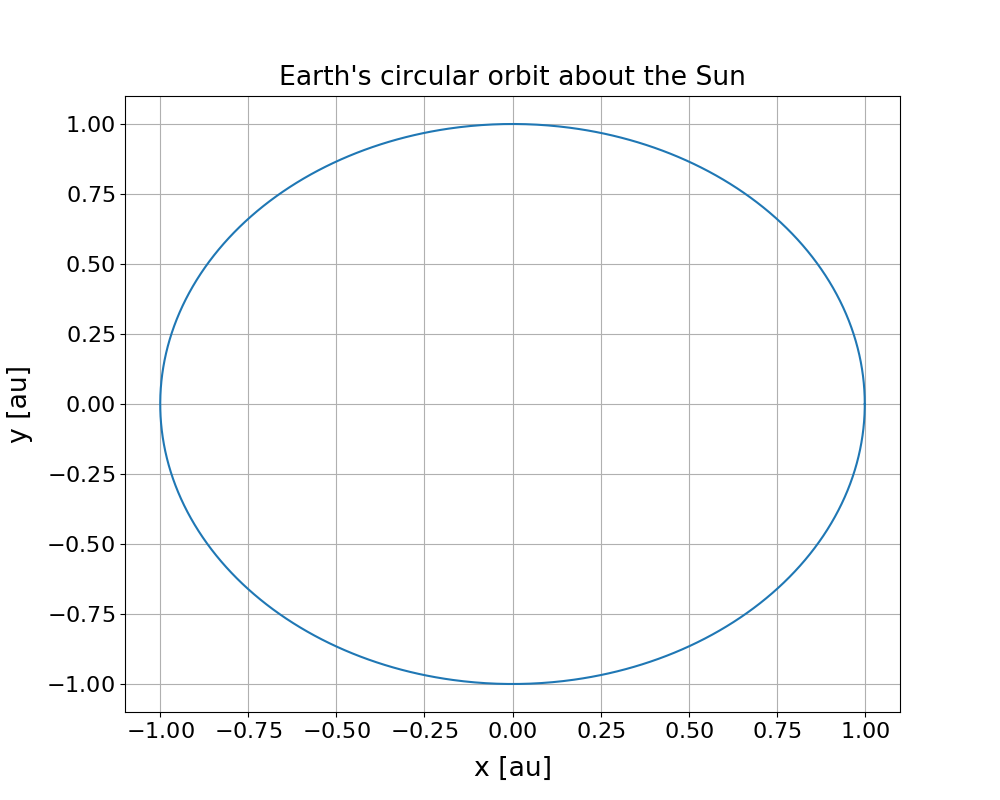
\includegraphics[scale=0.3]{../output/test_algorithms/Earth_orbit.png}
\caption{A plot of the two-dimensional simulation of Earth's orbit using initial conditions \(x=1\) au, \(y=0\) and an initial velocity equal to the ideal velocity for circular orbits.}\label{fig:Earth_orbit_circular}
\end{figure}

\begin{figure}[]
\centering
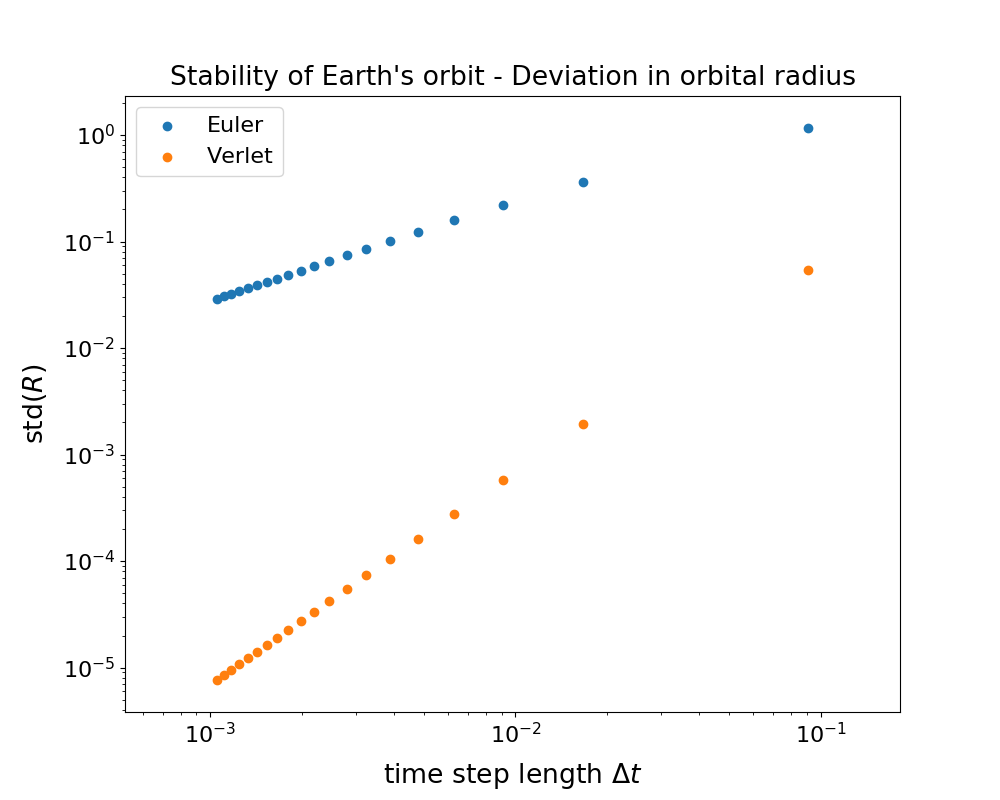
\includegraphics[scale=0.3]{../output/test_algorithms/Earth_Stability_radius.png}
\caption{The stability of Earth's orbit in the two-body Earth-Sun system, measured using the standard deviation in the orbit's radius \(|\vb{r}_i|\) with respect to the integration step length \(h\).}\label{fig:Earth_circular_stability_radius}
\end{figure}

\begin{figure}[]
\centering
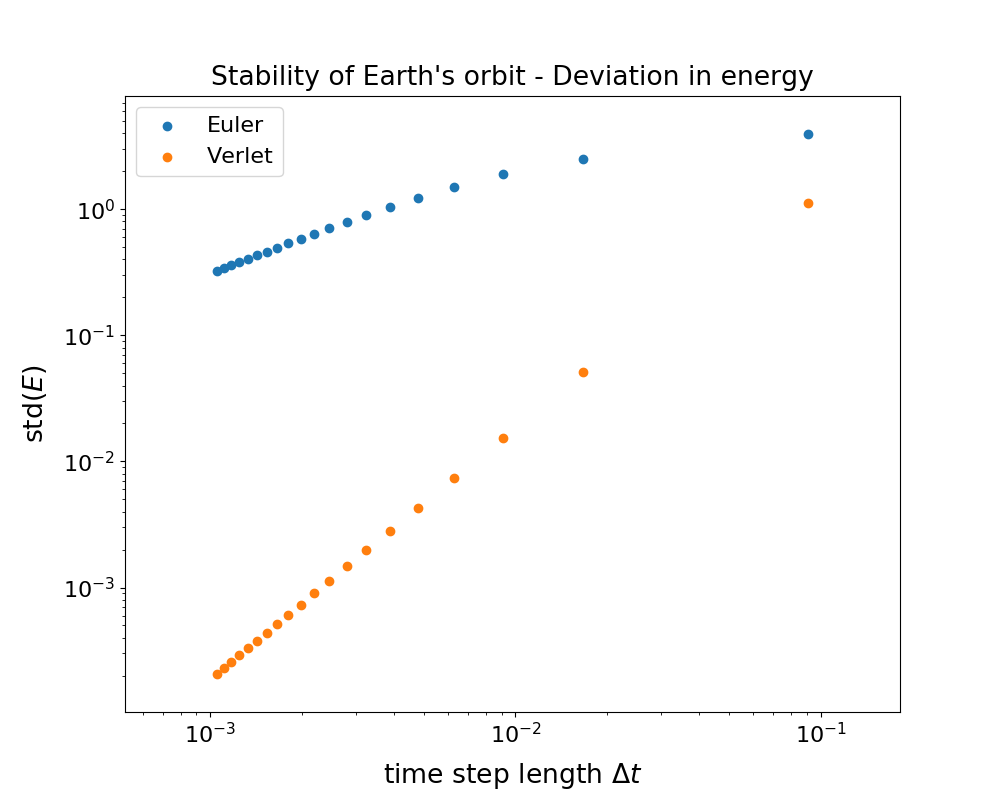
\includegraphics[scale=0.3]{../output/test_algorithms/Earth_Stability_energy.png}
\caption{The stability of Earth's orbit in the two-body Earth-Sun system, measured using the standard deviation in the orbit's mechanical energy \(E/M_E\) (equation \eqref{eq:mechanical_energy}) with respect to the integration step length \(h\).}\label{fig:Earth_circular_stability_energy}
\end{figure}

\begin{figure}[]
\centering
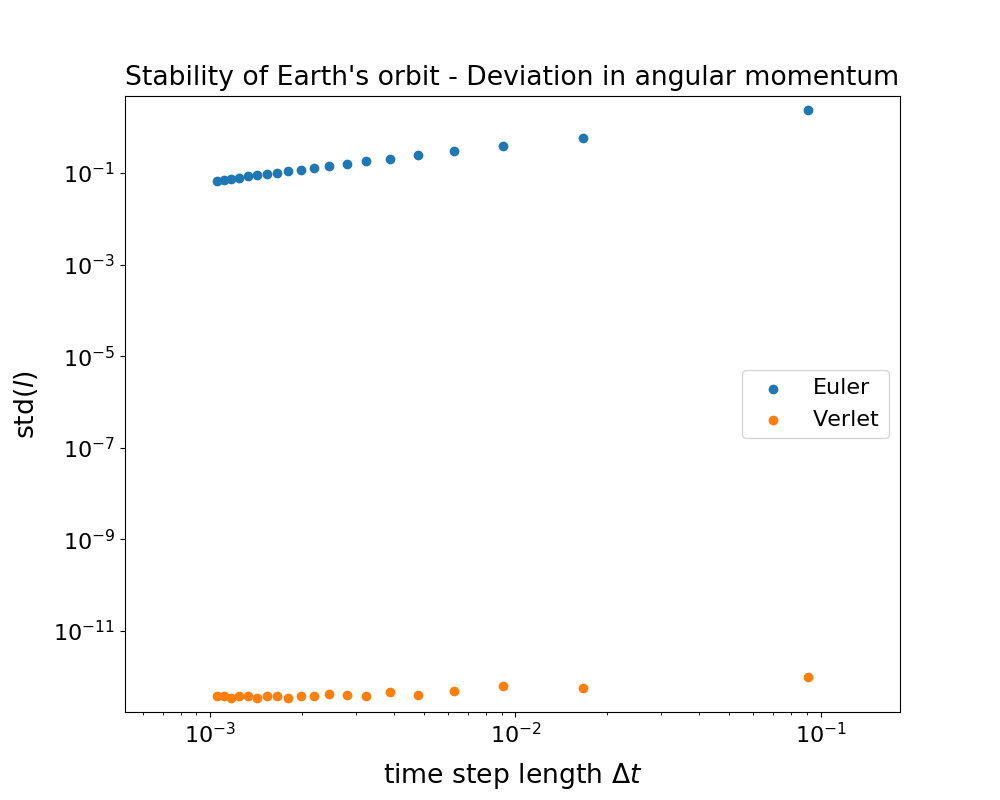
\includegraphics[scale=0.3]{../output/test_algorithms/Earth_Stability_angmom.png}
\caption{The stability of Earth's orbit in the two-body Earth-Sun system, measured using the standard deviation in the orbit's angular momentum \(l\) (equation \eqref{eq:angular_momentum}) with respect to the integration step length \(h\).}\label{fig:Earth_circular_stability_angmom}
\end{figure}

\newpage
\subsection{The Earth-Sun System: Escape Velocity}
Figure \ref{fig:Earth_escape_velocity} shows the effect of increasing the \(\beta\)-gravity parameter in \eqref{eq:beta_Newtonian_gravitational_acceleration} from 2 to 3. As Earth's initial velocity is kept constant, the gravitational attraction from the Sun for \(\beta>2\) is unable to trap Earth in its potential well. The simulations integrate the system using the Velocity-Verlet algorithm for 200 years with \(N=100\,000\) integration steps.
\begin{figure}[]
\centering
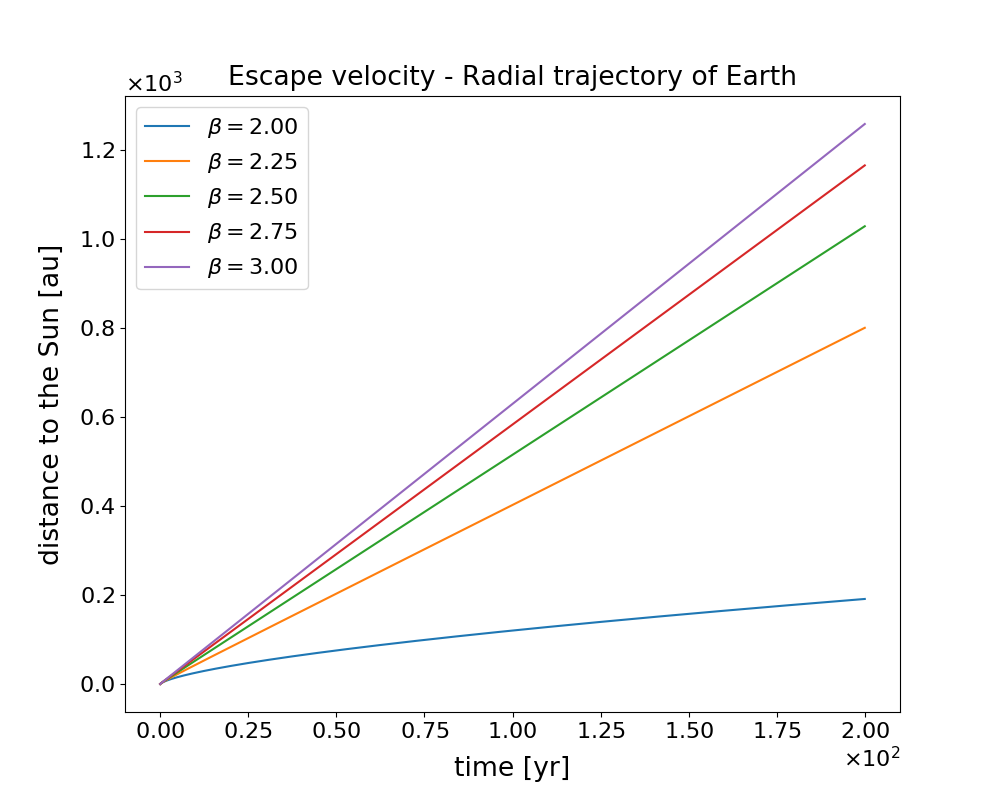
\includegraphics[scale=0.3]{../output/escape_velocity/radial_trajectory.png}
\caption{The effect of increasing the \(\beta\)-gravity parameter on the radial trajectory of Earth during a simulation of gravitational escape.}\label{fig:Earth_escape_velocity}
\end{figure}

\newpage
\subsection{The Earth-Jupiter-Sun System}
This three-body system was integrated 4 times using the Velocity-Verlet algorithm over the course of 2 years with \(N=200\,000\) integration steps. The first integration did not include Jupiter, while the 3 latter integrations included Jupiter with a mass of \(M_J\), \(10M_J\) and \(1000M_J\) respectively. The results are shown in figure \ref{fig:Earth_Jupiter_perturbation}. It is clear that Jupiter's standard perturbation of Earth's orbit is negligible. For the greater masses the effect does play a role as the radius begins to oscillate about a constant distance of 1. For the \(1000M_J\) case the motion is increasingly unstable as time continues, meaning the oscillation could increase to a point of significance in the long run.

\begin{figure}[]
\centering
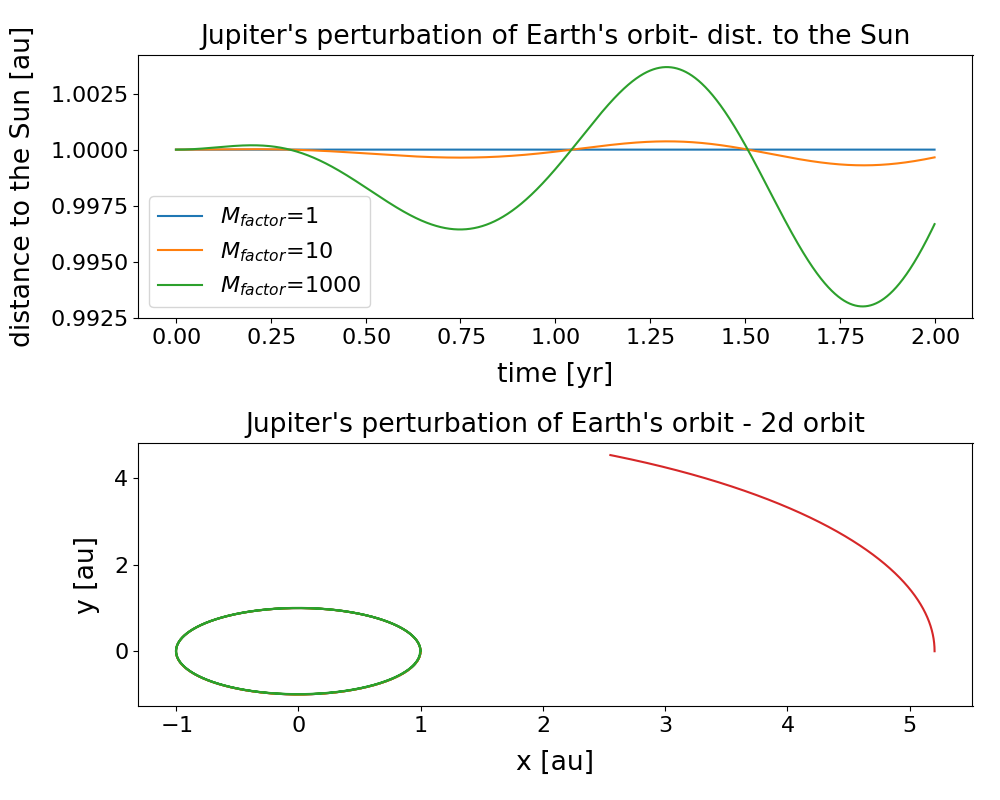
\includegraphics[scale=0.3]{../output/three_body_problem/Earth_perturbed_orbit.png}
\caption{Jupiter's perturbation of Earth's orbit about the Sun. The red orbit in the two-dimensional plot is Jupiter's orbit. All three Earth orbits are plotted in the two-dimensional plot.}\label{fig:Earth_Jupiter_perturbation}
\end{figure}
\subsection{The Solar System}
After many attempts, I declared myself unable to use the NASA data. I do not know if this is because I am reading the data wrong, the units wrong, or something entirely different. So I decided to use random generated initial conditions instead. I choose 8 uniformly distributed angles \(\theta\in[0,2\pi]\) and placed the planets in circular orbits according to \eqref{eq:circular_orbital_speed} using the "Distance to sun in AU" data from the project \texttt{pdf}. Then I gave the orbits a small disturbance in order to emulate perturbed orbits.

The system was run for 1 year using the Velocity-Verlet algorithm with \(N=500\,000\) integration steps, the results are shown below in figures \ref{fig:solar_system_2d} and \ref{fig:solar_system_3d}

\begin{figure}[]
\centering
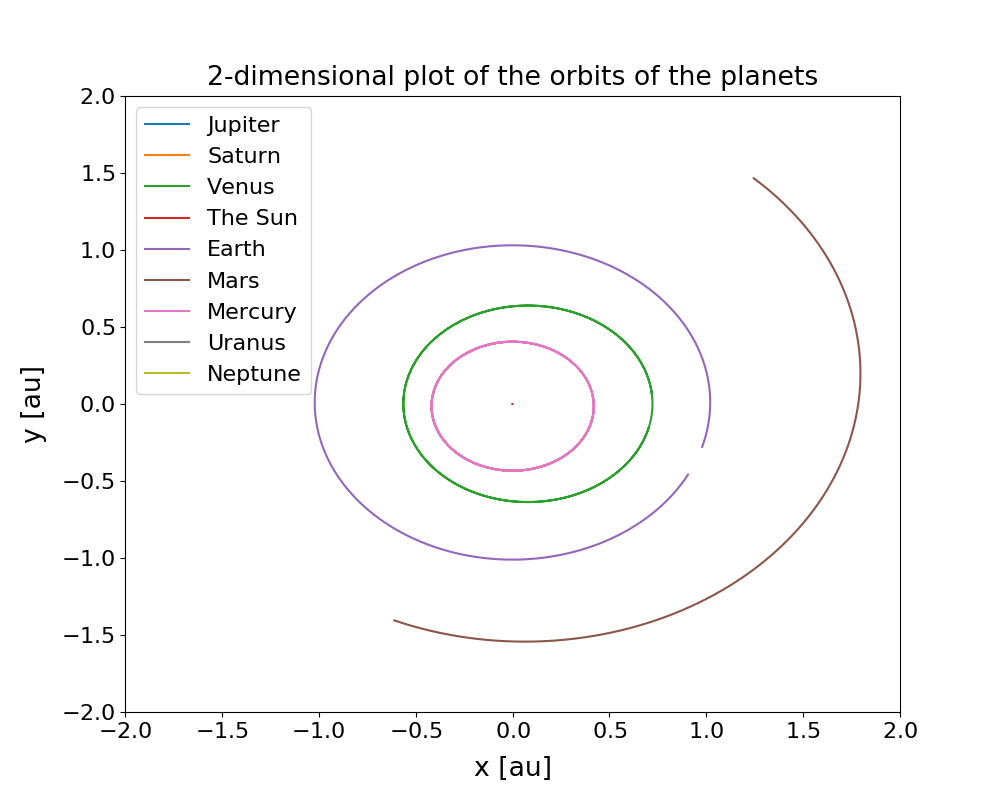
\includegraphics[scale=0.3]{../output/solar_system/solar_system_2d.png}
\caption{A two-dimensional plot of a three-dimensional simulation of the Solar System's planetary orbits. The initial conditions were randomised with inbedded pertubed orbits.}\label{fig:solar_system_2d}
\end{figure}

\begin{figure}[]
\centering
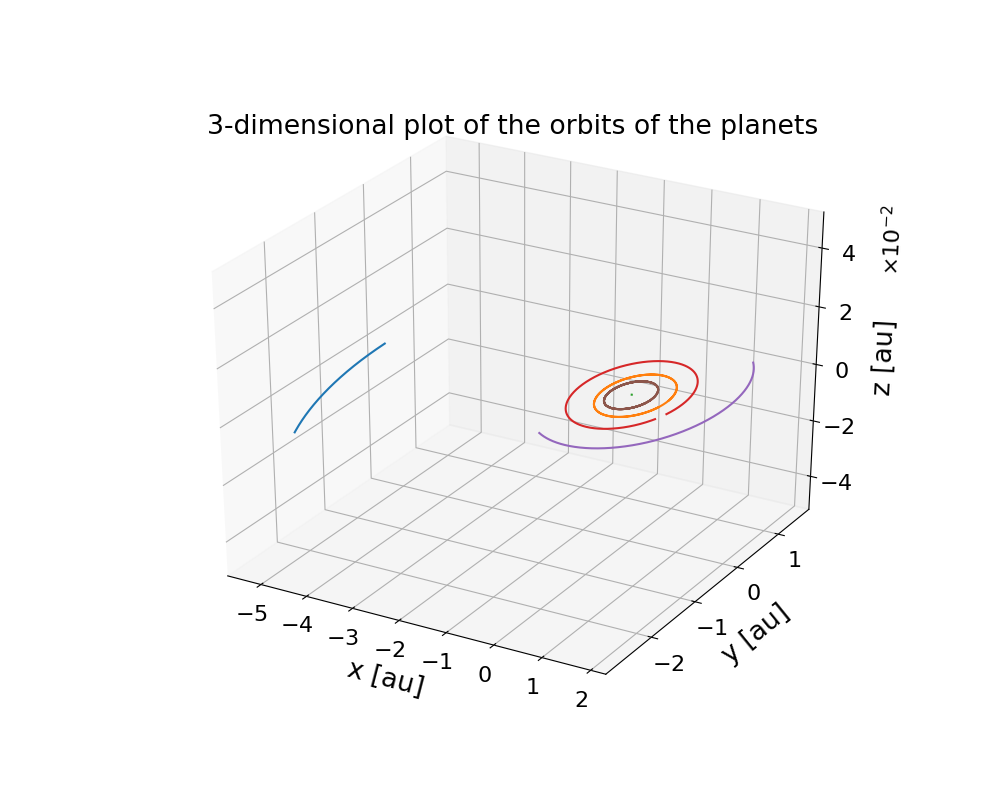
\includegraphics[scale=0.37]{../output/solar_system/solar_system_3d.png}
\caption{A plot of a simulation of the Solar System's planetary orbits. The initial conditions were randomised with inbedded pertubed orbits.}\label{fig:solar_system_3d}
\end{figure}

\subsection{The Perihelion Precession of Mercury}
Integrating the Mercury-Sun system using the Velocity-Verlet algorithm for 50 years with \(N=5\,000\,000\) integration steps yielded a total perihelion precession of 26.66'', which implies a shift of 53.31'' over the course of 100 years. Sadly this is a little to much compared to the expected shift 46'': an error of about 15.9\%. This is likely a result of an accumulative numerical error, which has increased to the point where its effects is of a significant order. 
\section{Discussion}
Dispite the success of the Velocity-Verlet algorithm in this report, the perihelion precesssion was reproduced with an of 15.9\%. One way to tackle this would be increase the number of integration points, however this solution fails once machine precision is reached. Another way would be to exchange the algorithm with a higher-order integration scheme, albeit it would also carry with it a greater number of computtions per simulation.


\section{Conclusion}
Overall, Project 3 has been a descent success. The Velocity-Verlet algorithm was shown, as expected, to be overly favoured over the simpler Forward-Euler algorithm. The Earth-Sun system (both the circular orbit scenario and the \(\beta\)-Newtonian escape-velocity scenario) behaved as predicted in the theory section. The perturbations of Earth's orbit due to the gravitational attraction from Jupiter were shown to have miniscule effects. On the other hand, the "10\(M_J\) Jupiter" instigated an oscillation in the orbital radius, while the "\(1000M_J\) Jupiter" drove the orbit unstable. The perihelion precession of Mercury was reproduced with an error of 15.9\%.

\bibliographystyle{plain}
\bibliography{references}
\end{document}
